\section{Supplementary results and reproducibility}
\label{app:supp}
\appendixnumbering

\figref{fig:mcbox} shows the box plots of fulfilment and total cost on the 52 operating days that underlie
\tabref{tab:mc}, and \figref{fig:sens0} repeats the sensitivity study of \figref{fig:sens} in the rule setting.
\tabref{tab:repro} lists, for every experiment, the script and the result files from which the tables and figures of this
paper are generated. All experiments run with GNU Octave 8.4 and glpk (or MATLAB with intlinprog or Gurobi through the
same interface); the complete set takes about 18~h in a single process or about 3~h in parallel batches, and the
smoke tests check that every optional feature leaves the base case unchanged when it is switched off.

\begin{figure*}[!t]
\centering
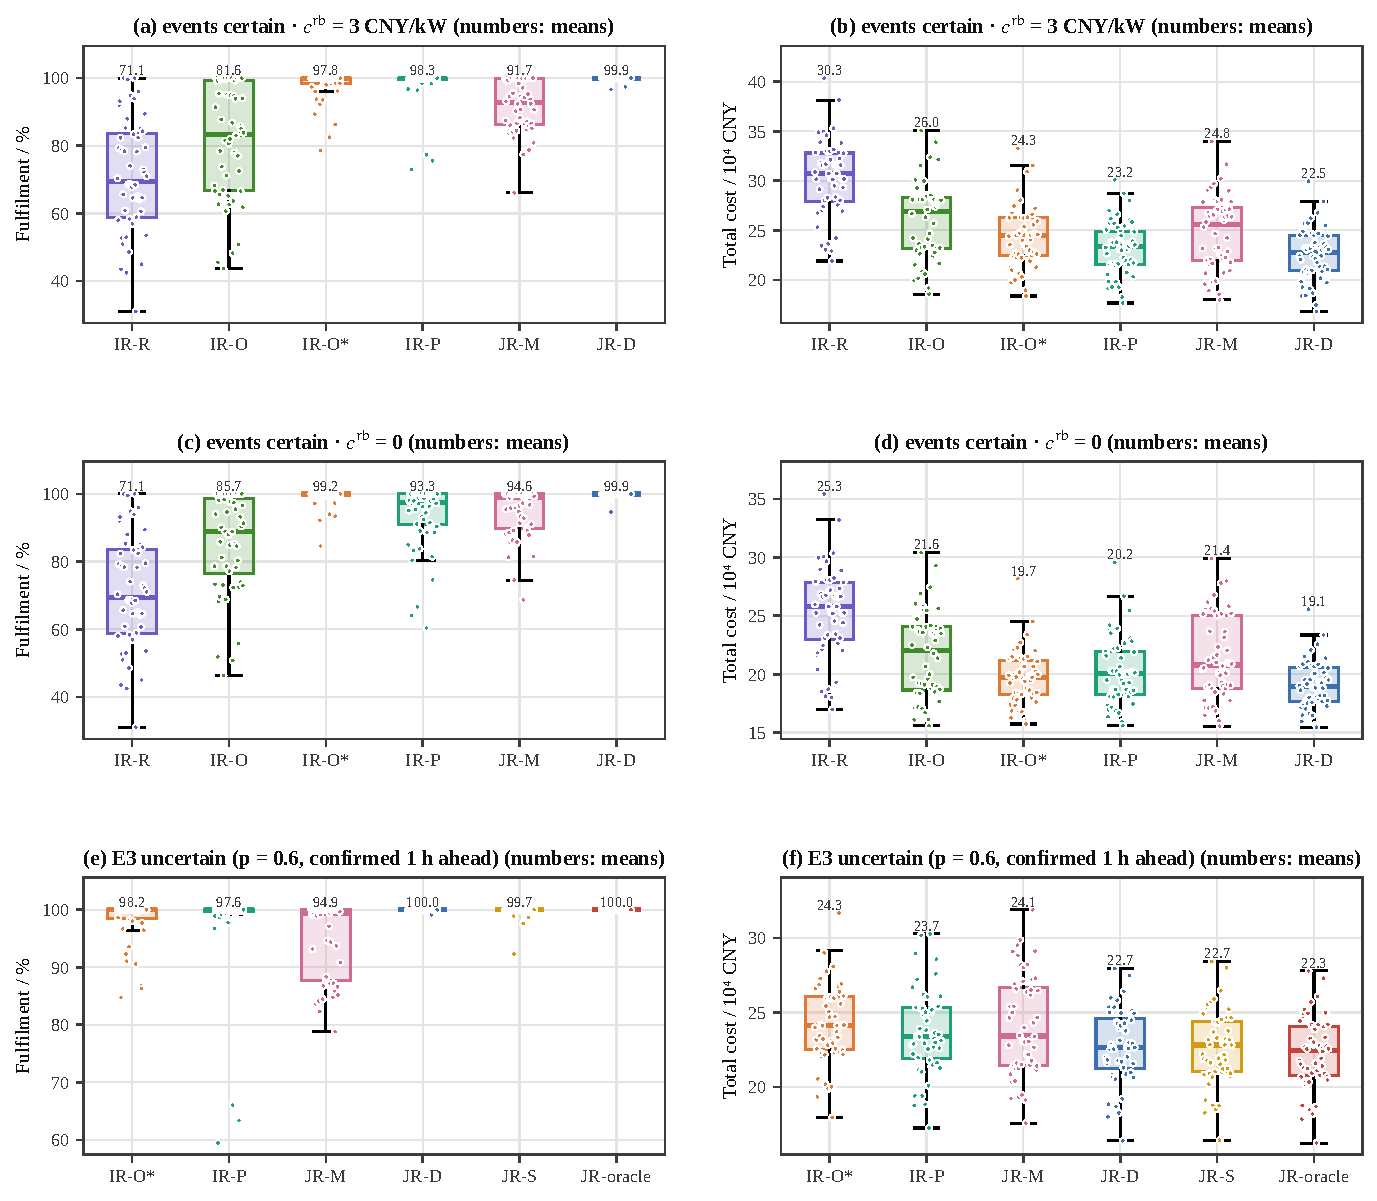
\includegraphics[width=0.86\textwidth]{fig07_montecarlo.pdf}
\caption{Fulfilment and total cost on the 52 operating days for the three settings (numbers: means).}
\label{fig:mcbox}
\end{figure*}

\begin{figure*}[!t]
\centering
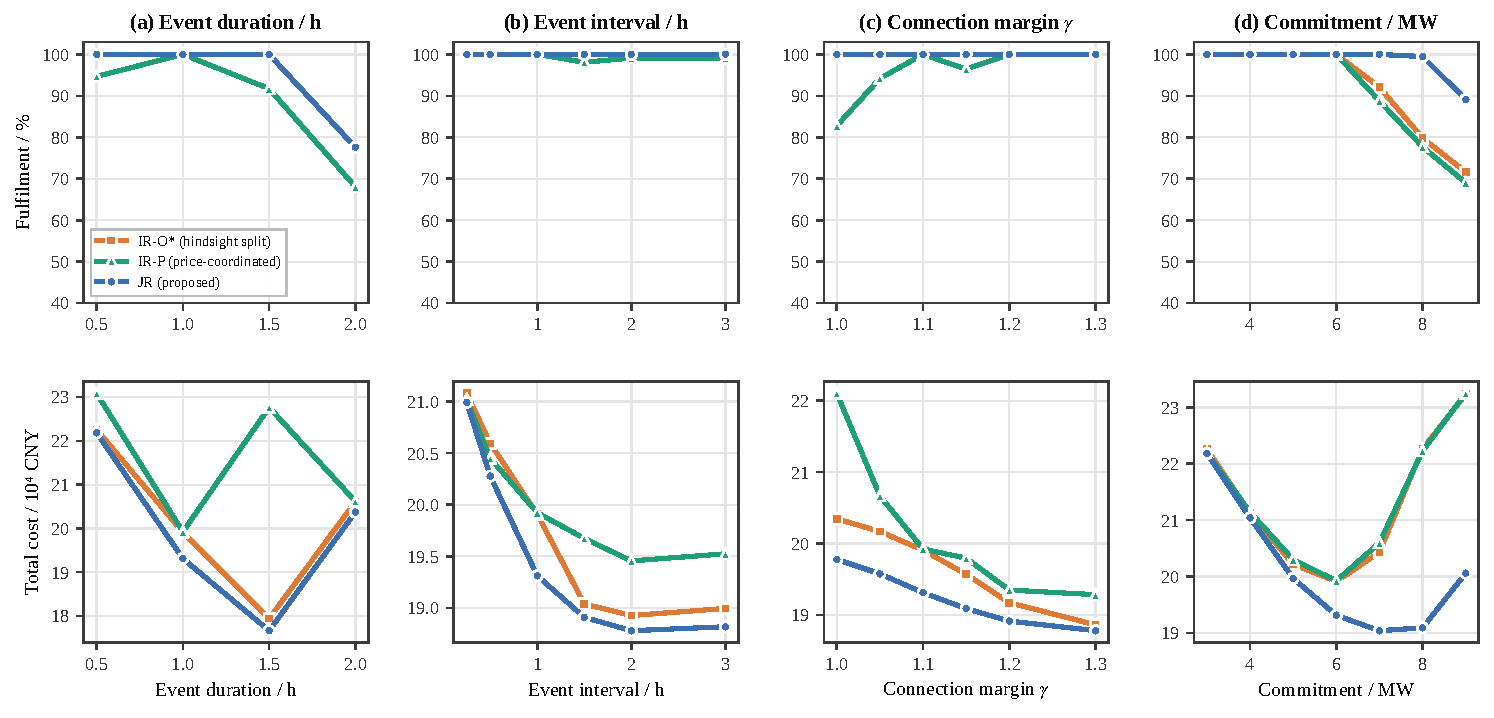
\includegraphics[width=0.96\textwidth]{fig05_sensitivity_crb0.pdf}
\caption{Sensitivity under perfect information in the rule setting ($\crb=0$): fulfilment (top) and total cost (bottom)
versus (a) event duration, (b) gap, (c) connection margin and (d) uniform commitment.}
\label{fig:sens0}
\end{figure*}

\begin{table*}[!t]
\caption{Experiments, scripts and result files (scripts in \texttt{matlab/experiments}, results in \texttt{matlab/results}).}
\label{tab:repro}
\centering\scriptsize
\setlength{\tabcolsep}{4pt}
\begin{tabularx}{\textwidth}{@{}c>{\raggedright\arraybackslash}p{0.16\textwidth}>{\raggedright\arraybackslash}p{0.19\textwidth}X@{}}
\toprule
No. & Experiment & Script & Result files\\
\midrule
1 & Mechanism & \texttt{exp1\_mechanism.m} & \texttt{exp1\_mechanism\_CA6\_DA2}, \texttt{exp1\_mechanism\_CA6\_DA1\_DB2}\\
2 & Case day & \texttt{exp2\_main.m} & \texttt{exp2\_\{DAcommit,uniform6\}[\_crb0]}, \texttt{exp2\_commitments}, \texttt{exp2\_alpha\_*}, \texttt{exp2\_lambda\_*}, \texttt{ts\_*}\\
3 & Sensitivity & \texttt{exp3\_sensitivity.m} & \texttt{exp3\_\{duration,interval,gamma,commitment,map\}[\_crb0]}\\
4 & 52 operating days & \texttt{exp4\_montecarlo.m} & \texttt{exp4\_\{certain,certain\_crb0,e3uncertain\}} with \texttt{\_strategies}, \texttt{\_bench}\\
5 & Shadow prices & \texttt{exp5\_shadow.m} & \texttt{exp5\_shadow*}, \texttt{exp5\_kkt*} (KKT residuals)\\
6 & Commitment pairing & \texttt{exp6\_commitment.m} & \texttt{exp6\_commitment[\_crb0]}, \texttt{exp6\_theta[\_crb0]}\\
7 & Ablation & \texttt{exp7\_ablation.m} & \texttt{exp7\_ablation}, \texttt{exp7\_alpha}\\
8 & Rebound charge & \texttt{exp8\_rebound.m} & \texttt{exp8\_rebound}, \texttt{exp8\_strategies}\\
9 & Payment $\times$ shortfall & \texttt{exp9\_price.m} & \texttt{exp9\_price}, \texttt{exp9\_strategies}\\
10 & Realism & \texttt{exp10\_realism.m} & \texttt{exp10\_realism}\\
11 & Theorem 1 & \texttt{exp11\_stylized.m} & \texttt{exp11\_stylized}\\
12 & Reliable capacity & \texttt{exp12\_capacity.m} & \texttt{exp12\_capacity\_crb0}, \texttt{exp12\_strategies\_crb0}\\
13 & Substitution & \texttt{exp13\_substitution.m} & \texttt{exp13\_substitution}, \texttt{exp13\_strategies}\\
14 & Timing & \texttt{exp14\_timing.m} & \texttt{exp14\_timing}\\
15 & Risk-averse commitment & \texttt{exp15\_risk.m} & \texttt{exp15\_commit}, \texttt{exp15\_oos}, \texttt{exp15\_settings}\\
16 & Tariff shapes & \texttt{exp16\_tariff.m} & \texttt{exp16\_tariff}, \texttt{exp16\_tariff\_mc}, \texttt{exp16\_shapes}\\
17 & Policy and coupling & \texttt{exp17\_policy.m} & \texttt{exp17\_policy}, \texttt{exp17\_strategies}\\
18 & Climate & \texttt{exp18\_climate.m} & \texttt{exp18\_climate}, \texttt{exp18\_climate\_mc}, \texttt{exp18\_cases}\\
19 & Job-level validation & \texttt{exp19\_workload.m} & \texttt{exp19\_workload\_\{pai,acme\}\_\{fluid,rigid\}}, \texttt{exp19\_variants}, \texttt{ts\_job\_*}\\
20 & Job mix and overheads & \texttt{exp20\_jobsim.m} & \texttt{exp20\_jobsim}, \texttt{exp20\_settings}, \texttt{exp20\_strategies}\\
21 & Offshore wind & \texttt{exp21\_wind.m} & \texttt{exp21\_curve}, \texttt{exp21\_wind}, \texttt{exp21\_strategies}\\
22 & Overheads and capping & \texttt{exp22\_overhead.m} & \texttt{exp22\_overhead\_\{a,b,c\}}, \texttt{exp22\_settings}\\
23 & Scenario generation & \texttt{exp23\_scenarios.m} & \texttt{exp23\_commit}, \texttt{exp23\_oos}, \texttt{exp23\_settings}\\
24 & Waste-heat recovery & \texttt{exp24\_heat.m} & \texttt{exp24\_heat}, \texttt{exp24\_settings}, \texttt{ts\_heat\_*}\\
25 & Capability region & \texttt{exp25\_region.m} & \texttt{exp25\_\{case,radial,vertices,irp,slices,sweep,mc,irp\_eps\}}\\
26 & Distributed coordination & \texttt{exp26\_admm.m} & \texttt{exp26\_\{conv,ref,price\}}, \texttt{exp26\_mc}, \texttt{exp26\_rho}, \texttt{exp26\_strategies}\\
\bottomrule
\end{tabularx}
\end{table*}
